\documentclass[a4paper]{article}

\usepackage[english, swedish]{babel}
\usepackage{float}
\usepackage{minted}
\usepackage[style=ieee]{biblatex}
\usepackage{csquotes}
\usepackage[toc,title]{appendix}
\usepackage{titlesec}
\usepackage{hyperref}
\usepackage{url}
\usepackage{graphicx}

\graphicspath{{images/}}


\hypersetup{
    colorlinks,
    citecolor=black,
    filecolor=black,
    linkcolor=black,
    urlcolor=black
}

\renewcommand\appendixtocname{Bilagor}


\addbibresource{references.bib}

\begin{document}
\pagenumbering{gobble}

\begin{titlepage}
    \centering

    \vspace*{0,5cm}

    \begin{LARGE}
        \textbf{Gymnasiearbete Handroid}
    \end{LARGE}

    \begin{Large}

        \vspace{1cm}

        Spårning och representation av fingerrörelser.

    \end{Large}

    \vspace{1cm}

    \begin{large}
        Gabriel Calota\\
        Jonathan Damsgaard Falck\\
        William Johansson
    \end{large}

    \vspace{0.5cm}
    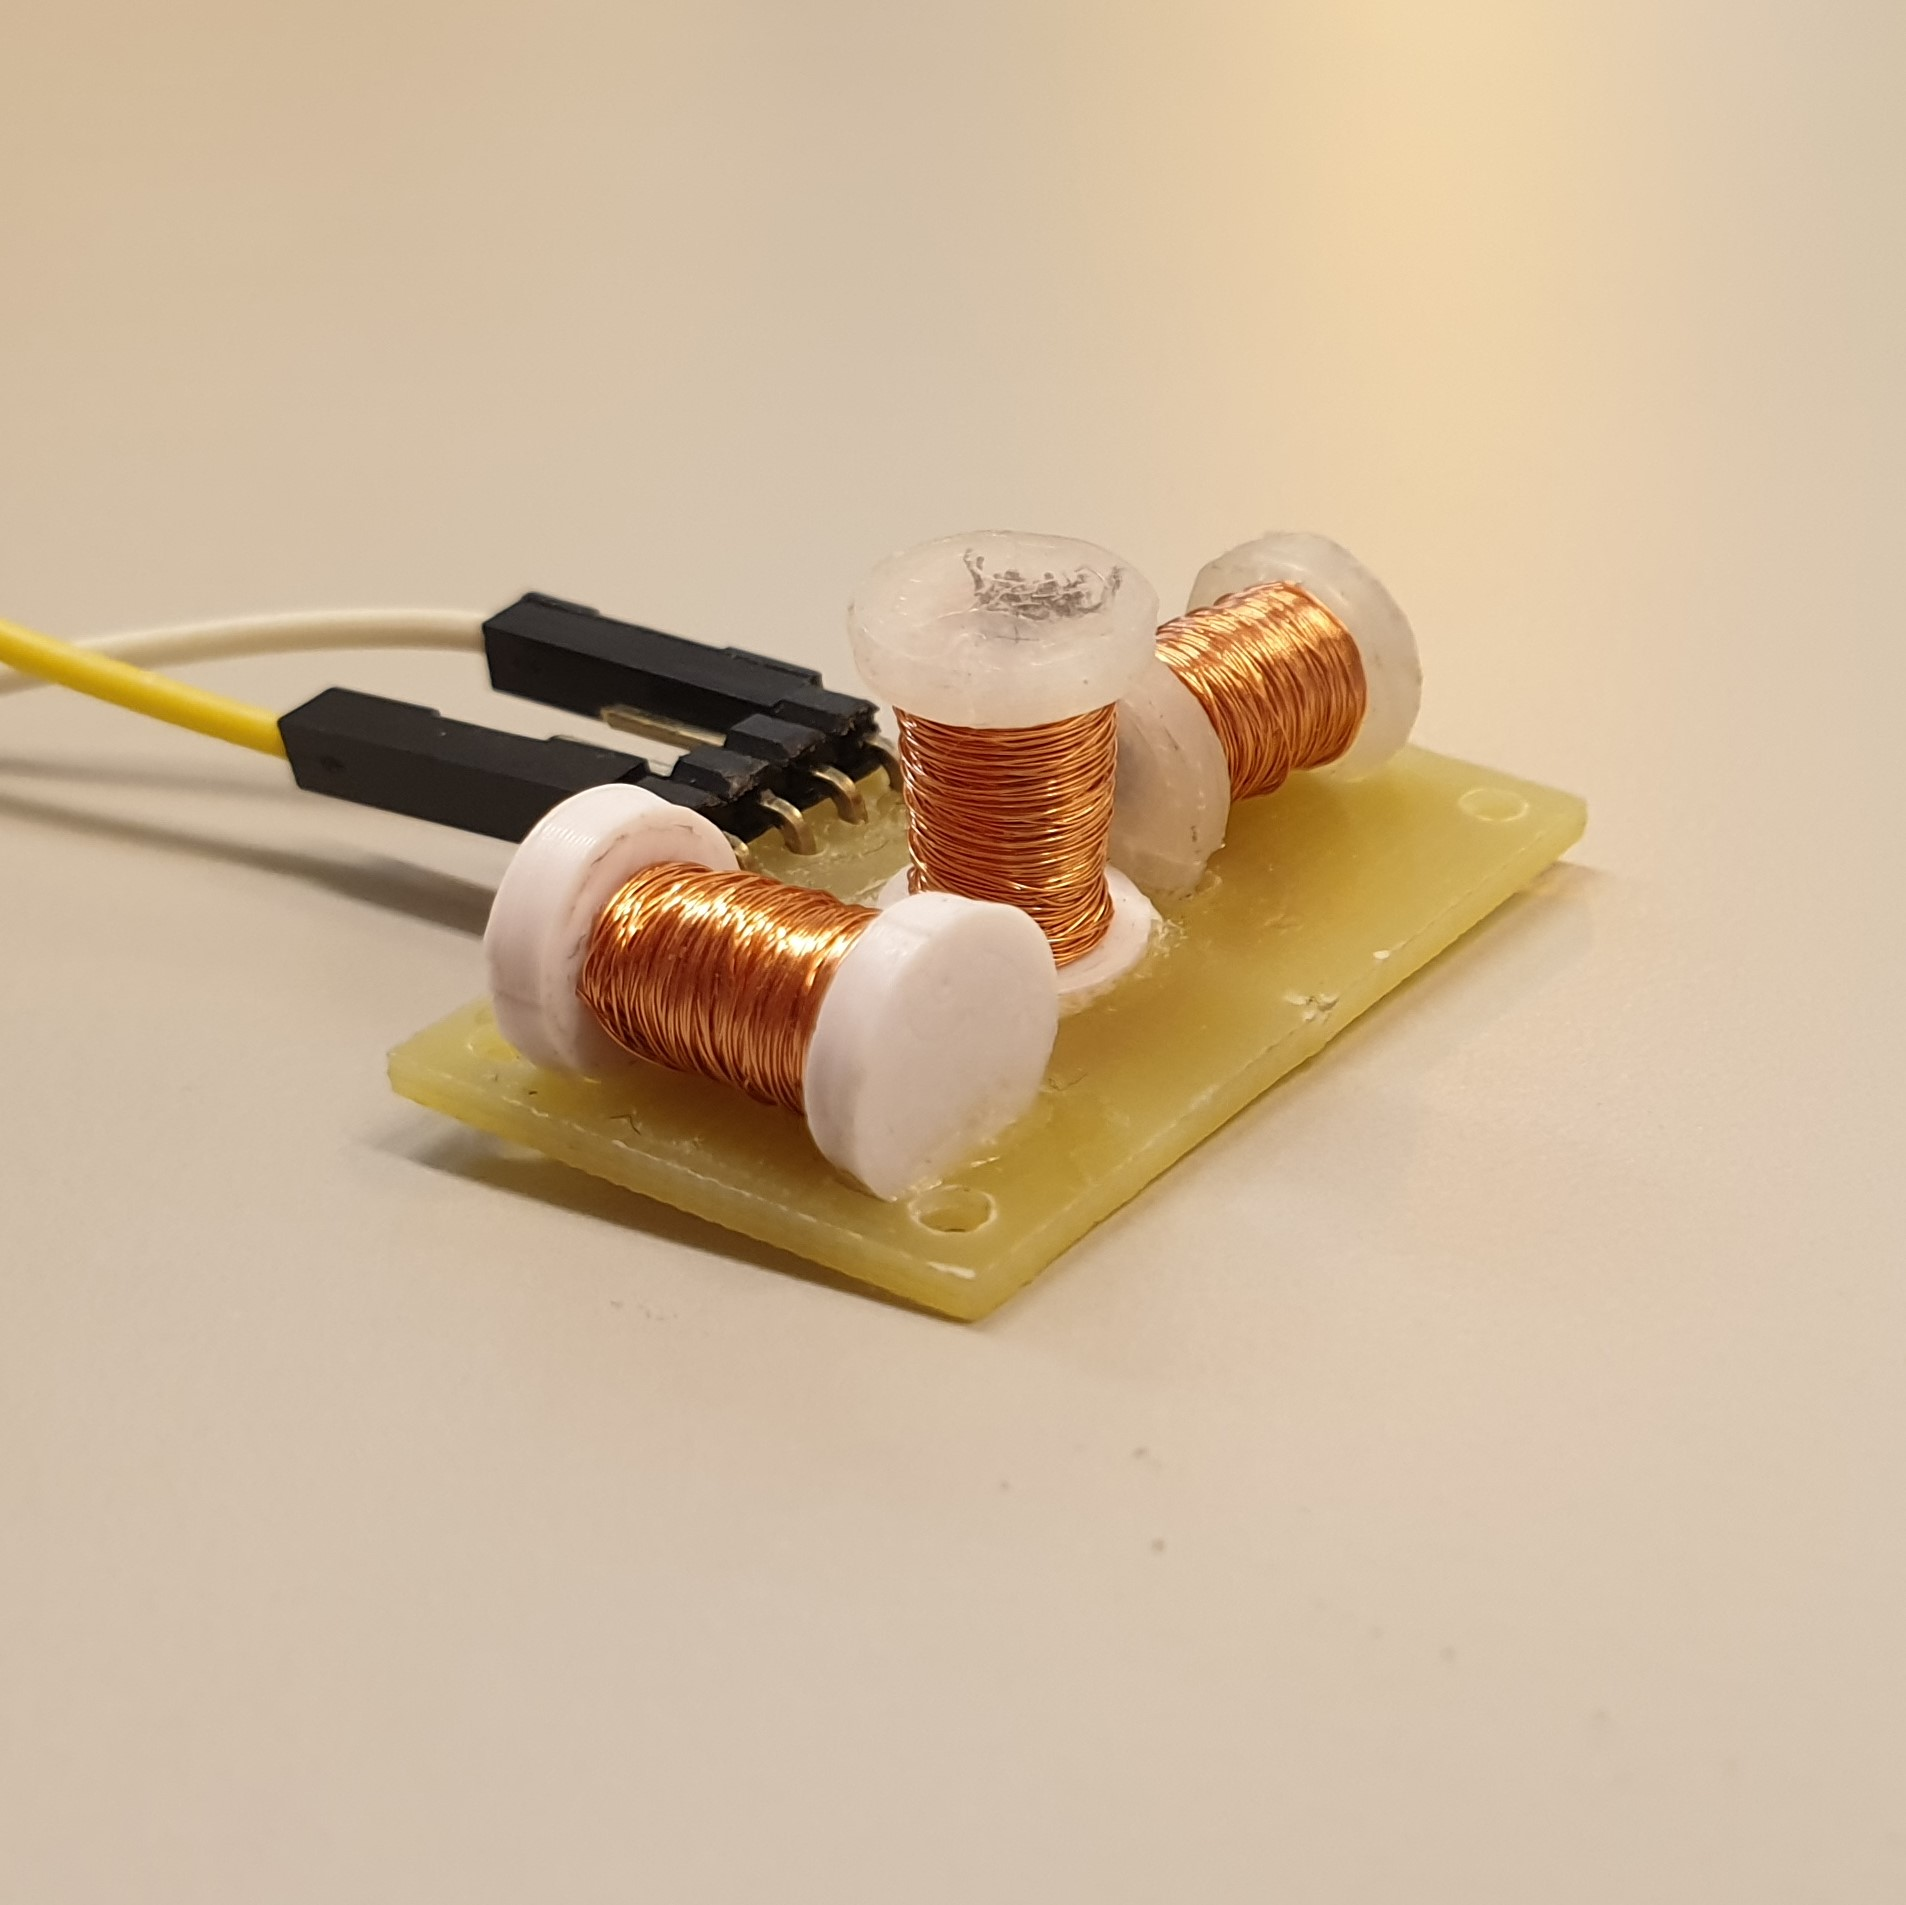
\includegraphics[width=\textwidth]{images/Spolhubb1.jpg}
    \vfill

    \begin{large}
        Lärosäte: ABB-Gymnasiet\\
        \vspace{0.5cm}
        Klass: 190S\\
        \vspace{0.5cm}
        Handledare: Andreas Jillram, ABB-Gymnasiet
    \end{large}

\end{titlepage}


\begin{abstract}

\end{abstract}

\begin{otherlanguage}{english}
    \begin{abstract}
    \end{abstract}
\end{otherlanguage}

\tableofcontents

\newpage
\pagenumbering{arabic}

\begin{sloppypar}

    \section{Inledning}
    \subsection{Syfte}
    Syftet med projektet är att undersöka hur människan finmotoriska rörelser kan detekteras, hur rörelserna såsom fingerrörelse kan användas som inmatning till olika system
    och utveckla ett prototyp som kan både detektera och återskapa fingerrörelser på en människohand.
    De finmotoriska rörelser kan återskapas antingen med en digital representation av rörelsen eller med en fysisk robothand.
    % De detekterade rörelserna ska sedan översättas till data som går att visualisera exempelvis genom att kontrollera en fysisk robothand eller digitalt i ett datorprogram.
    \subsection{Bakgrund}
    Det finns ett ökat intresse och en ökad efterfrågan på olika sätt för människan att interagera med datorer och robotar.
    Bland annat hur människokroppen kan användas för inmatning till datorprogram och till olika maskiner.
    Den här tekniken är som mest utvecklad inom virtual reality och augmented reality och det är inom dessa områden som tekniken i nuläget har störst användning.
    Tekniken är dock fortfarande relativt begränsad och använder mestadels grövre motorik som inmatning och förlorar den precision som kan ges av finmotoriska rörelser.

    % Vi ser ett ökande intresse för andra applikationer där människan agerar fjärrkontroll.   

    \subsection{Frågeställning}

    \section{Teori}
    För att få en bättre bild av hur en robothand kan skapas och styras med hjälp av olika sensorer undersöktes andra, liknande projekt.
    Projektet drog inspiration från en kandidatexamen från två KTH-studenter~\cite{KTHhand} med ett liknande syfte, och
    idéer för tummens funktion på den fysiska handen kom från ett projekt som hette \textit{Etho Hand}~\cite{EthoHand}
    vars syfte var att utveckla en hand som kunde utföra komplexa rörelser.


    \subsection{Elektromagnetism}
    \subsubsection{Magnetfält}
    Magnetfält är fält som rör sig i en riktning från nord- till sydpolen på en magnet eller runt en strömförande elektrisk ledare.
    Den magnetiska flödestätheten, ekvivalent med magnetfältets \textit{styrka}, kring en ledare med ström, avtar med avstånd från ledaren,
    vilket är relevant för detta projekt.~\cite{digilar}
    \subsubsection{Induktion}
    Inducerad spänning är spänning som alstras när en ledare befinner sig i ett magnetfält, på grund av att de laddade partiklarna hamnar på motsatta sidor av ledaren.
    Det skapar en skillnad i laddning, vilket korrelerar med spänning.
    Enligt Lenz lag ger denna spänning upphov till en ström, i en sluten krets, och att strömmens riktning motverkar förändringen av det magnetiska flödet.
    Denna princip kan användas för att alstra ström ur ett magnetfält, exempelvis i en generator.
    Induktion fungerar också åt motsatt håll: ström och spänning i en krets ger upphov till magnetfält runt ledaren.
    ~\cite{digilar}

    \subsection{Elektronik}
    \subsubsection{Spolar}
    En spole är en ledare som lindats i varv på ett sådant sätt att magnetfältet som skapas när ström flödar igenom har en nord- och en sydpol.
    Spolar kan lindas runt ett material, en \textit{kärna} som förstärker magnetfältet, eller bara med luft i mitten.
    På grund av att spolen inducerar spänning kommer den motverka strömmen i kretsen den ingår, enligt Lenz lag, vilket bland annat ger en förskjutning mellan spänning och ström, i en växelströmskrets.~\cite{digilar}
    \subsubsection{Mätning av spolar}
    För att dimensionera en krets kan det vara viktigt att veta vilka värden ens komponenter har.
    Till restistorer och kondensatorer är detta oftast enkelt, då de flesta moderna multimetrarna kan mäta resistans och kapacitans.
    Verktyg för att mäta spolars induktans (som mäts i enheten 1 Henry) är sällsyntare, och därför finns olika metoder för att själv mäta spolar utan specialverktyg.
    För detta kan exempelvis en funktionsgenerator och ett oscilloskop användas, och genom att utnyttja spolens upp- och urladdningsförmåga kan man med hjälp av matematiska formler approximera spolens induktans.~\cite{MeasureInductor}

    \subsubsection{Kondensatorer}
    Kondensatorn är en elektrisk komponent som kan lagra elektrisk energi, genom att laddas upp och laddas ur med spänning, vilket ger upphov till en förskjutning mellan ström och spänning, i en växelströmskrets.~\cite{digilar}

    \subsubsection{Operationsförstärkare}
    \subsubsection{Filter}
    \subsubsection{Oscillatorer}
    En oscillator är en elektrisk krets eller en del av en elektrisk krets där växelström, ström som regelbundet byter riktning, skapas.
    På grund av spolars och kondensatorers upp- och urladdningsförmåga kan dessa användas, i olika kombinationer för att göra en krets där strömmen och spänningen svänger (blir svagare/starkare, och byter riktning) med en viss frekvens.
    Oscillatorer är användbara om man vill skapa växelström med en likströmskälla, vilket för det här projektet är mycket relevant för att kunna alstra ett varierande magnetfält i spolarna.

    En sorts oscillator är en Wien-bryggeoscillator (\textit{Wien Bridge Oscillator})~\cite{WienBridge} där resistorer, kondensatorer och en operationsförstärkare används för att skapa en vågformad växelströmssignal, där frekvensen bestäms av resistorernas och kondensatorernas värden.
    En annan sorts oscillator är en 555-oscillator~\cite{555_sine}, som bygger på ett chip med en integrerad krets (\textit{IC}) vid namn 555. 555-chippet kan ge fyrkantsformade utsignaler om de sätts i ett visst värde, och där frekvensen bestäms med hjälp av restistorer och kondensatorer. Det går också att filtrera signalen så att den liknar en sinusvåg, med hjälp av en spole och kondensatorer.


    \subsubsection{Flexsensorer}
    En flexsensor är en sensor som ändrar resistans proportionerligt med hur mycket den är böjd.
    Flexsensorer kan användas för att mätta gur mycket ett finger är böjd och de har använts i projekt och produkter som ... .
    \subsubsection{Accelerometer}
    \subsubsection{Mikrokontroller}
    \subsubsection{Arduino Nano 33 BLE}
    Arduino Nano 33 BLE är en mikrokontroller baserad på kretsen Nordic nRF52480 producerad av företaget Arduino.
    Arduino Nano 33 BLE är en fysiskt liten mikrokontroller. Nordic nRF52480 är bestyckad med en Cortex M4F processor
    och en NINA B306 BLE-modul som möjliggör kommunikation med Bluetooth Low Energy. Arduino Nano 33 BLE har 8 analoga
    ingångar och kan drivas av spänning mellan 4,5 och 21 volt. Annan viktig hårdvaruinformation om mikrokontrollern
    kan ses i tabell~\ref{table:ArduinoNano}. ~\cite{Arduino:ABX00030}\\\
    Mikrokontrollern används för att läsa av mätvärden från sensorerna och för att skicka vidare mätvärdena till
    datorn där renderingen sker. Den programmeras i C++ med hjälp av platformIO, en tillbyggnad i utvecklingsmiljön
    Visual Studio Code som möjliggör programmering av mikrokontrollers i C++. 

    \begin{table}[h]
        \begin{center}
            \caption{Viktiga specifikationer Arduino Nano 33 BLE ~\cite{Arduino:ABX00030}}
            \label{table:ArduinoNano}
            \begin{tabular}{ | l | l | }
                \hline
                Mikrokontroller            & nRF52840 \\
                \hline
                Driftspänning              & 3,3V     \\
                \hline
                Inspänning (min)           & 4,5V     \\
                \hline
                Inspänning (max)           & 21V      \\
                \hline
                Digitala ingångar/utgångar & 14 st    \\
                \hline
                Analoga ingångar           & 8 st     \\
                \hline
                Längd                      & 45 mm    \\
                \hline
                Bredd                      & 18 mm    \\
                \hline
            \end{tabular}
        \end{center}
    \end{table}
    \subsubsection{555-timer}
    \subsection{Bluetooth Low Energy}
    Bluetooth Low Energy liknar traditionell Bluetooth, men är mer energieffektiv.
    \subsubsection{Peripheral}
    \subsubsection{Central}

    \subsection{Rendering}
    \subsubsection{Unity}
    Unity är en programvara som möjliggör skapandet av real-time 3d-miljöer för spel, film etc. https://unity.com/our-company.

    \section{Metod och material}



    \subsection{Konstruktion}

    \subsubsection{3D-hand}
    En design för en fysisk 3D-hand skapades som skulle kontrolleras av fingerdetektionen.
    Designen bestod av servon som med hjälp av trådar styr fingrarna
    och 3d-modeller av fingersegment som kunde skrivas ut med en 3D-skrivare.

    \subsubsection{Spolar}
    Spolar användes för att skapa och läsa av magnetfältet som används för att läsa av fingrets position och rotation.
    En spole består av en järnkärna, 0,1 mm koppartråd samt 3D-printade hattar
    För att få lämplig storlek och funktion från spolarna valdes ett varvtal på 1000 varv.
    Spolarna konstruerades genom att limma fast hattar i ändarna på järnkärnan.
    Sedan lindades spolarna med koppartråd.
    Lindningen gjordes genom att fästa den olindade spolen i en motor som genom att snurra samtidigt som koppartråd
    var fäst i den olindade spolen gjorde att järnkärnan lindades med koppartråden.
    Motorn var kopplad till en Arduino mikrokontroller som med hjälp av en varvmätare kunde läsa av hur många varv
    koppartråd som hade lindats runt spolen.
    När mikrokontrollern räknat att motorn roterat 1000 varv stängdes motorn automatiskt av. Se figur \ref{fig:Spolsnurrare}.


    \begin{figure}[h]
        \centering
        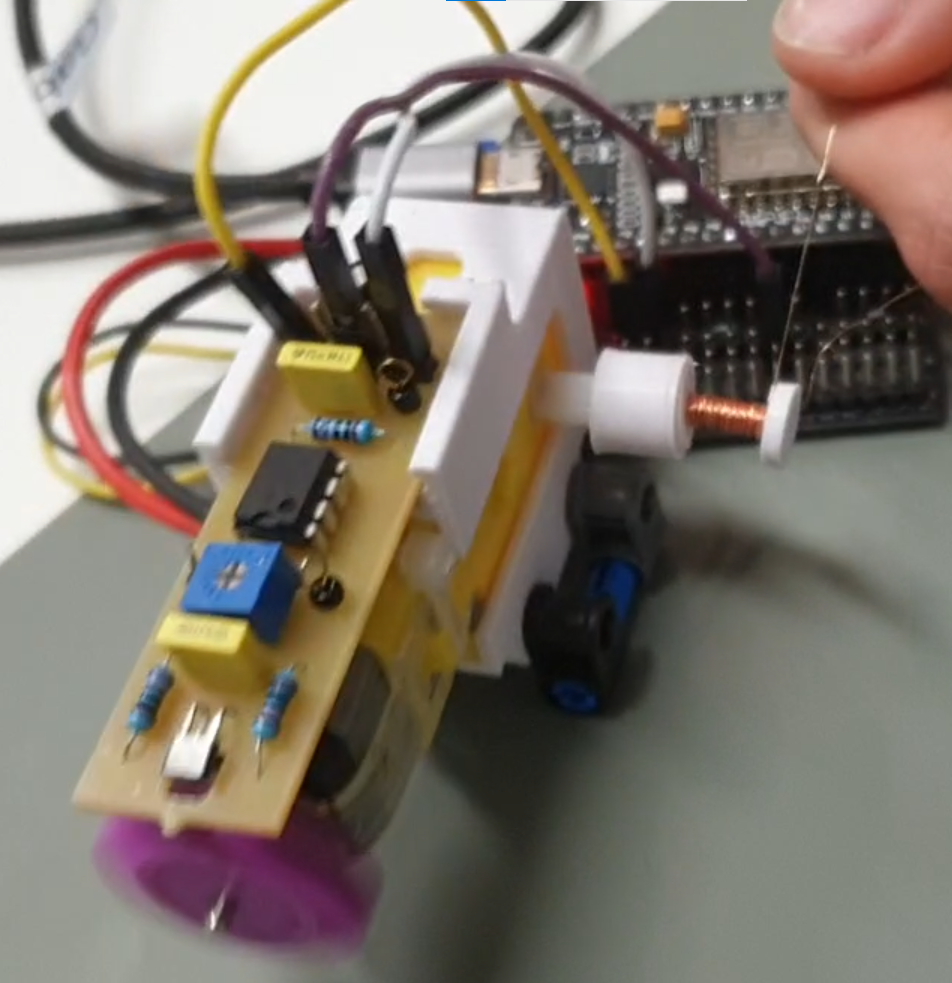
\includegraphics[width=0.75\textwidth]{spolsnurrare1.png}
        \caption{Bild från när en spole lindades med hjälp av Spolsnurraren.}
        \label{fig:Spolsnurrare}
    \end{figure}
    
    För att få bättre kontakt med andra kablar och komponenter valdes ett antal spolar ut för att lödas fast i kablar av större tjocklek.
    Jämförelsen mellan en spole med fastlödd kabel och en spole utan fastlödd kabel kan ses i figur \ref{fig:SpoleVsSpole}.

    \begin{figure}[h]
        \centering
        \includegraphics[width = 0.75\textwidth]{spole-vs-spole.jpg}
        \caption{En spole med endast hatt, kärna och lindning (överst) och en spole med kablar fastlödda (underst).}
        \label{fig:SpoleVsSpole}
    \end{figure}


    \subsubsection{Montering på hand} %3d prints,  etc. bättre titel
    För att montera spolar på handen monterades de tre mottagarspolarna på ett kretskort som agerade spolhubb.
    De tre spolarna monterades i varsin riktning så att de kan ta upp fingerrörelser i tre dimensioner.
    Kretskortet modellerades i ultiboard och frästes sedan ut på skolan kretskortsfräs.
    På kretskortet monterades spolarna genom att limmas fast i kretskorten och koppartråden löddes fast på kortets undersida.
    För att kunna skicka vidare signalen som spolarna plockar upp löddes även en stiftlist fast på kretskortet.


    \subsection{Kretsar}
    \subsubsection{Filter}
    Filtret ska filtrera frekvenser som inte är inom ett visst frekvensområde och ett aktivt bandpassfilter valdes som filtertyp.
    Filterkretsen designades först med hjälp av formler för att bestämma värden på kondensatorer och resistorer.
    Kretsen testades sedan i simulering för att säkerställa att kretsens fungerar som förväntat,
    dock användes en ideal operationsförstärkare under simuleringen.
    När kretsen sedan simulerades med icke-ideal operationsförstärkare kunde kretsen inte längre filtrera signalen.
    Det visades sig att formlerna för kondensatorer och resistorer
    antog att operationsförstärkare var ideal för att kretsen skulle fungera.
    Kretsen designades sedan om med hjälp av ett filter designverktyg av Texas Instruments
    och fungerade i simulering med en icke-ideal operationsförstärkare.
    \subsubsection{Oscillator}


    \subsection{Rendering}
    \subsubsection{Mikrokontroller}
    Mikrokontrollen Arduino Nano 33 BLE används för att kommunicera med renderingsprogrammet.
    Mikrokontrollen väntar på renderingsprogrammet att ansluta och
    läser sedan av värdena från de olika sensorerna och publicerar dessa till en Bluetooth characteristics.
    För att åstadkomma kommunikation används biblioteket ArduinoBLE.

    \subsubsection{Renderingsprogram}
    Renderingsprogrammet som används är Unity.
    För att kommunicera med mikrokontrollen används BleWinrtDll och hand modellen kommer från Ultraleaps Unity Plugin.
    Programmet översätter värdena från sensorerna till rotationer i fingrarnas leder.





    \section{Resultat}
    \section{Diskussion och Slutsats}
    \subsection{Diskussion}

    \subsection{Slutsats}

    \section{Avslutning}




    \section{Källor}
    \printbibliography[heading=none]

    \appendices
    \titleformat{\section}[display]
    {\normalfont\Large\bfseries}{\appendixname\enspace\thesection}{.5em}{} %ny rad efter bilaga x
    \section{Renderingskod}

    \section{Oscillatorkrets}
    images/555-117kHz (Bild läggs in senare)
    bild på själva breadborden kanske?


    \section{Filterkrets}

    \section{Kod Spolsnurrare}
    \inputminted[]{cpp}{./Code/Spolsnurrare.cpp}
    \newpage
\end{sloppypar}


\end{document}